\documentclass[border=12pt]{standalone}
\usepackage{tikz}
\usetikzlibrary{arrows,positioning,shapes.geometric}
\begin{document}


\tikzset{every picture/.style={line width=0.75pt}} %set default line width to 0.75pt        

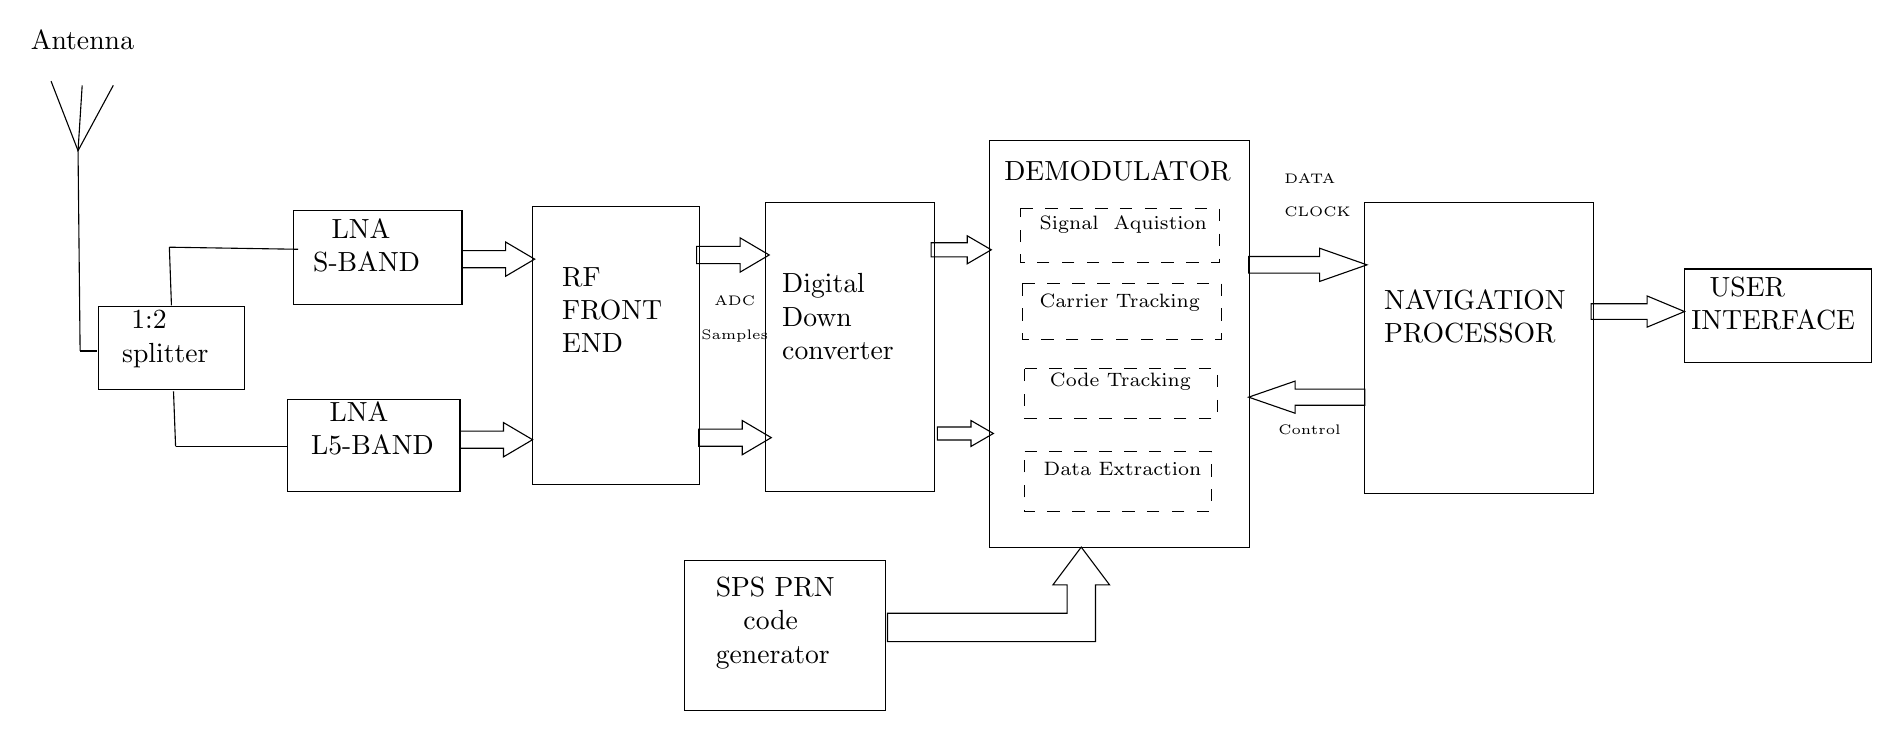
\begin{tikzpicture}[x=0.75pt,y=0.75pt,yscale=-1,xscale=1]
%uncomment if require: \path (0,418); %set diagram left start at 0, and has height of 418

%Shape: Rectangle [id:dp91775771381591] 
\draw   (38,182) -- (108,182) -- (108,222) -- (38,222) -- cycle ;
%Shape: Rectangle [id:dp6878402250141991] 
\draw   (132,136) -- (213,136) -- (213,181) -- (132,181) -- cycle ;
%Shape: Rectangle [id:dp44768197824429146] 
\draw   (129,227) -- (212,227) -- (212,271) -- (129,271) -- cycle ;
%Shape: Rectangle [id:dp5655754137730491] 
\draw   (247,134) -- (327.5,134) -- (327.5,268) -- (247,268) -- cycle ;
%Shape: Rectangle [id:dp570158544072791] 
\draw   (359,132) -- (440.5,132) -- (440.5,271) -- (359,271) -- cycle ;
%Shape: Rectangle [id:dp6780374126781124] 
\draw   (467,102) -- (592.5,102) -- (592.5,298) -- (467,298) -- cycle ;
%Shape: Rectangle [id:dp38178392589317034] 
\draw   (648,132) -- (758,132) -- (758,272) -- (648,272) -- cycle ;
%Shape: Rectangle [id:dp48587293841162293] 
\draw   (802,164) -- (892,164) -- (892,209) -- (802,209) -- cycle ;
%Shape: Rectangle [id:dp527299782431056] 
\draw  [dash pattern={on 4.5pt off 4.5pt}] (482,135) -- (578,135) -- (578,161) -- (482,161) -- cycle ;
%Shape: Rectangle [id:dp25121868516157364] 
\draw  [dash pattern={on 4.5pt off 4.5pt}] (483,171) -- (579,171) -- (579,198) -- (483,198) -- cycle ;
%Shape: Rectangle [id:dp7112717721020039] 
\draw  [dash pattern={on 4.5pt off 4.5pt}] (484,212) -- (577,212) -- (577,236) -- (484,236) -- cycle ;
%Shape: Rectangle [id:dp6802603568978252] 
\draw  [dash pattern={on 4.5pt off 4.5pt}] (484,252) -- (574,252) -- (574,281) -- (484,281) -- cycle ;
%Right Arrow [id:dp3847468665289855] 
\draw   (757,180.75) -- (784,180.75) -- (784,177) -- (802,184.5) -- (784,192) -- (784,188.25) -- (757,188.25) -- cycle ;
%Right Arrow [id:dp11379212184339593] 
\draw   (592,158) -- (626.2,158) -- (626.2,154) -- (649,162) -- (626.2,170) -- (626.2,166) -- (592,166) -- cycle ;
%Left Arrow [id:dp3964692546932914] 
\draw   (592,225.75) -- (614.4,218) -- (614.4,221.88) -- (648,221.88) -- (648,229.63) -- (614.4,229.63) -- (614.4,233.5) -- cycle ;
%Right Arrow [id:dp047248875449849015] 
\draw   (213,155.13) -- (234,155.13) -- (234,151) -- (248,159.25) -- (234,167.5) -- (234,163.38) -- (213,163.38) -- cycle ;
%Straight Lines [id:da16506188383170162] 
\draw    (28,107) -- (29,203.5) ;
%Straight Lines [id:da053092707540165485] 
\draw    (29,203.5) -- (37,203.5) ;
%Straight Lines [id:da7479103158784801] 
\draw    (15,73.5) -- (28,107) ;
%Straight Lines [id:da023170939991778106] 
\draw    (30,75.5) -- (28,107) ;
%Straight Lines [id:da6039548016175794] 
\draw    (28,107) -- (45,75.5) ;
%Straight Lines [id:da397178408511075] 
\draw    (72,153.5) -- (134,154.5) ;
%Straight Lines [id:da6398771401584881] 
\draw    (72,153.5) -- (73,181.5) ;
%Straight Lines [id:da8993427310127735] 
\draw    (74,223) -- (75,249.5) ;
%Straight Lines [id:da5504549537888844] 
\draw    (75,249.5) -- (129,249.5) ;
%Right Arrow [id:dp38901755194750065] 
\draw   (212,242.13) -- (233,242.13) -- (233,238) -- (247,246.25) -- (233,254.5) -- (233,250.38) -- (212,250.38) -- cycle ;
%Right Arrow [id:dp9617272144769732] 
\draw   (326,153.13) -- (347,153.13) -- (347,149) -- (361,157.25) -- (347,165.5) -- (347,161.38) -- (326,161.38) -- cycle ;
%Right Arrow [id:dp24676205787927274] 
\draw   (327,241.13) -- (348,241.13) -- (348,237) -- (362,245.25) -- (348,253.5) -- (348,249.38) -- (327,249.38) -- cycle ;
%Right Arrow [id:dp7057810479841495] 
\draw   (439,151.38) -- (456.4,151.38) -- (456.4,148) -- (468,154.75) -- (456.4,161.5) -- (456.4,158.13) -- (439,158.13) -- cycle ;
%Right Arrow [id:dp5533926878537673] 
\draw   (442,240.13) -- (458.2,240.13) -- (458.2,237) -- (469,243.25) -- (458.2,249.5) -- (458.2,246.38) -- (442,246.38) -- cycle ;
%Shape: Rectangle [id:dp6070084344522547] 
\draw   (320,304.5) -- (417,304.5) -- (417,376.5) -- (320,376.5) -- cycle ;
%Bend Up Arrow [id:dp7529447413881465] 
\draw   (418,329.85) -- (504.53,329.85) -- (504.53,316.2) -- (497.7,316.2) -- (511.35,298) -- (525,316.2) -- (518.18,316.2) -- (518.18,343.5) -- (418,343.5) -- cycle ;

% Text Node
\draw (490,137) node [anchor=north west][inner sep=0.75pt]   [align=left] {{\scriptsize Signal \ Aquistion }};
% Text Node
\draw (490,175) node [anchor=north west][inner sep=0.75pt]   [align=left] {{\scriptsize Carrier Tracking}};
% Text Node
\draw (495,213) node [anchor=north west][inner sep=0.75pt]   [align=left] {{\scriptsize Code Tracking }};
% Text Node
\draw (492,256) node [anchor=north west][inner sep=0.75pt]   [align=left] {{\scriptsize Data Extraction}};
% Text Node
\draw (473,111) node [anchor=north west][inner sep=0.75pt]   [align=left] {DEMODULATOR};
% Text Node
\draw (656,173) node [anchor=north west][inner sep=0.75pt]   [align=left] {NAVIGATION\\PROCESSOR};
% Text Node
\draw (804,167) node [anchor=north west][inner sep=0.75pt]   [align=left] { \ \ USER\\INTERFACE};
% Text Node
\draw (608,117) node [anchor=north west][inner sep=0.75pt]   [align=left] {{\tiny DATA }\\{\tiny CLOCK}};
% Text Node
\draw (605,238) node [anchor=north west][inner sep=0.75pt]   [align=left] {{\tiny Control}};
% Text Node
\draw (366,165) node [anchor=north west][inner sep=0.75pt]   [align=left] {Digital\\Down\\converter \\};
% Text Node
\draw (260,162) node [anchor=north west][inner sep=0.75pt]   [align=left] {RF\\FRONT \\END};
% Text Node
\draw (139,227) node [anchor=north west][inner sep=0.75pt]   [align=left] { \ \ LNA \\L5-BAND};
% Text Node
\draw (140,139) node [anchor=north west][inner sep=0.75pt]   [align=left] { \ \ LNA\\S-BAND};
% Text Node
\draw (48,183) node [anchor=north west][inner sep=0.75pt]   [align=left] { \ 1:2\\splitter};
% Text Node
\draw (327,176) node [anchor=north west][inner sep=0.75pt]   [align=left] {{\tiny  \ \ ADC}\\{\tiny Samples}};
% Text Node
\draw (4,48) node [anchor=north west][inner sep=0.75pt]   [align=left] {Antenna};
% Text Node
\draw (334,311.5) node [anchor=north west][inner sep=0.75pt]   [align=left] {SPS PRN \\ \ \ \ code \\generator};


\end{tikzpicture}

\end{document}
